\documentclass[12pt]{article}
\usepackage[a4paper, margin=1in]{geometry} 
\usepackage{graphicx} 
\usepackage{hyperref}
\usepackage{float}
\usepackage{multicol}
\usepackage{multirow}
\usepackage{amsmath}
\usepackage[ruled]{algorithm2e}
\usepackage{amssymb}
\usepackage[font=small, labelfont=bf]{caption}
\usepackage[table,xcdraw]{xcolor}

\title{Lecture Notes for \\ INF281 Basics of Bioinformatics Sequence Analysis}
\author{Takaya Saito}
\date{}

\begin{document}

\pagenumbering{arabic}
\setcounter{page}{59}

\makeatletter 
\renewcommand{\thefigure}{\arabic{section}.\arabic{figure}}
\renewcommand{\thetable}{\arabic{section}.\arabic{table}}
\makeatother

%
% PART IV
%
\setcounter{part}{3}
\part{}

%
% Multiple sequence alignment
%
\setcounter{section}{7}
\setcounter{figure}{0}
\setcounter{table}{0}
\section{Multiple sequence alignment}
%\documentclass[12pt]{article}
%\usepackage[a4paper, margin=1in]{geometry} 
%\usepackage{graphicx} 
%\usepackage{hyperref}
%\usepackage{float}
%\usepackage{multicol}
%\usepackage{multirow}
%\usepackage{amsmath}
%\usepackage[font=small, labelfont=bf]{caption}
%
%\begin{document}

%
% Multiple sequence alignment
%
\subsection{Multiple sequence alignment}
A multiple sequence alignment is an effective tool to understand the characteristics of genes by comparing multiple sequences of different species at the same time.

%
% Multiple Sequence Alignment (MSA) for protein sequences
%
\subsubsection*{Multiple Sequence Alignment (MSA) for protein sequences}
\begin{figure}[H]
  \centering
      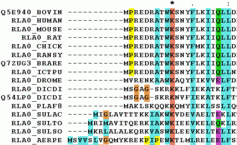
\includegraphics[width=0.3 \textwidth]{fig08/msa_part.png}
  \caption{An MSA of insulin proteins of seven sequences}
\end{figure}

%
% Notation of MSA
%
\subsubsection*{Notation of MSA}
\begin{itemize}
\item $\mathcal{A}$ : Alignment
\item $m$ : Number of sequences in $\mathcal{A}$
\item $s_j^i$ : An amino acid or a nucleotide of sequence $i$ and position $j$ (without gaps)
\item $\bar{s}_j^i$ : An amino acid or a nucleotide of sequence $i$ and column $j$ (with gaps)
\end{itemize}

%
% Example of MSA notation
%
\subsubsection*{Example of MSA notation}
\begin{verbatim}
    HUMAN: TP-K
    MOUSE: TLSK
    RAT  : TPSK
\end{verbatim}

\begin{itemize}
\item $m$ :	3
\item $s_1^1$ : T (1st position of HUMAN)
\item $s_2^2$ : L (2nd position of MOUSE)
\item $s_4^3$ : K (4th position of RAT)
\item $\bar{s}_3^1$ : - (3rd position of HUMAN)
\end{itemize}

%
% Making an optimal MSA
%
\subsubsection*{Making an optimal MSA} 

\begin{itemize}
\item Insert gaps to the sequences in $\mathcal{A}$
\item Maximize the score of $\mathcal{A}$
\end{itemize}

%
% All combinations of elements per column
%
\subsubsection*{All combinations of elements per column} 
The number of all possible combinations of elements per column can be calculated as follows.

\[
\sum_{i=0}^{m-1} \binom{m}{i}  = 2^m - 1
\]

%
% Example of the number of combinations
%
\subsubsection*{Example of the number of combinations} 

\begin{table}[H]
\begin{tabular}{ccccccc}
$s_1^1$ & - & $s_3^1$ & $s_4^1$ & - & - & $s_7^1$ \\
$s_1^2$ & $s_2^2$ & - & $s_4^2$ & - & $s_6^2$ & - \\
$s_1^3$ & $s_2^3$ & $s_3^3$ & - & $s_5^3$ & - & -                     
\end{tabular}
\end{table}

\begin{itemize}
\item $m$: 3
\item $2 \times 2 \times 2 - 1 = 7$
\end{itemize}

%
% Alignment methods
%
\subsubsection*{Alignment methods} 

\begin{itemize}
\item Dynamic programming with $m$-dimensional array (deterministic)
\item Progressive alignment (heuristics)
\end{itemize}

%
% SP score
%
\subsubsection*{SP score} 
One of the common methods to calculate the score of an alignment is using SP (sum-of-pairs) scores. SP uses pair-wise scores on all possible paired sequences to obtain the final score for the alignment. SP is defined as below.

\[
S(\mathcal{A}) = \sum_{i=1}^{m-1} \sum_{j=i+1}^{m} S(\bar{s}^i, \bar{s}^j)
\]

\textbf{N.B.} The score of $S(\bar{s}^i, \bar{s}^j)$ is 0 when both elements are gaps.

%
% Example of SP score
%
\subsubsection*{Example of SP score} 
Use the simple scoring scheme and calculate the SP score. Simple scoring scheme: Match: 1, Mismatch: 0, and Gap penalty: 1

\begin{verbatim}
    Seq1 A-GC
    Seq2 ACG-
    Seq3 A-TC
\end{verbatim}

\noindent
$S(\bar{s}^1, \bar{s}^2)=1-1+1-1=0$ \\
$S(\bar{s}^1, \bar{s}^3)=1+0+0+1=2$ \\
$S(\bar{s}^2, \bar{s}^3)=1-1+0-1=-1$ \\

\noindent
$S(\mathcal{A}) =S(\bar{s}^1, \bar{s}^2) + S(\bar{s}^1, \bar{s}^3) + S(\bar{s}^2, \bar{s}^3) = 0 + 2 - 1 = 1$

%
% Exercise \thesection.1
%
\subsubsection*{Exercise \thesection.1}
Use the simple scoring scheme and calculate the SP score.

\begin{verbatim}
    Seq1 A-CC
    Seq2 C-TC
    Seq3 CAG-
\end{verbatim}

\bigskip 

%\end{document}

%\documentclass[12pt]{article}
%\usepackage[a4paper, margin=1in]{geometry} 
%\usepackage{graphicx} 
%\usepackage{hyperref}
%\usepackage{float}
%\usepackage{multicol}
%\usepackage{multirow}
%\usepackage{amsmath}
%\usepackage[font=small, labelfont=bf]{caption}
%
%\begin{document}

%
% Multiple sequence alignment
%
\subsection{Dynamic programming with $m$-dimensional array}
Dynamic programming (DP) can be extended to handle multiple alignments. 

%
% Multi-dimensional array for dynamic programming
%
\subsubsection*{Multi-dimensional array for dynamic programming}
\begin{figure}[H]
  \centering
      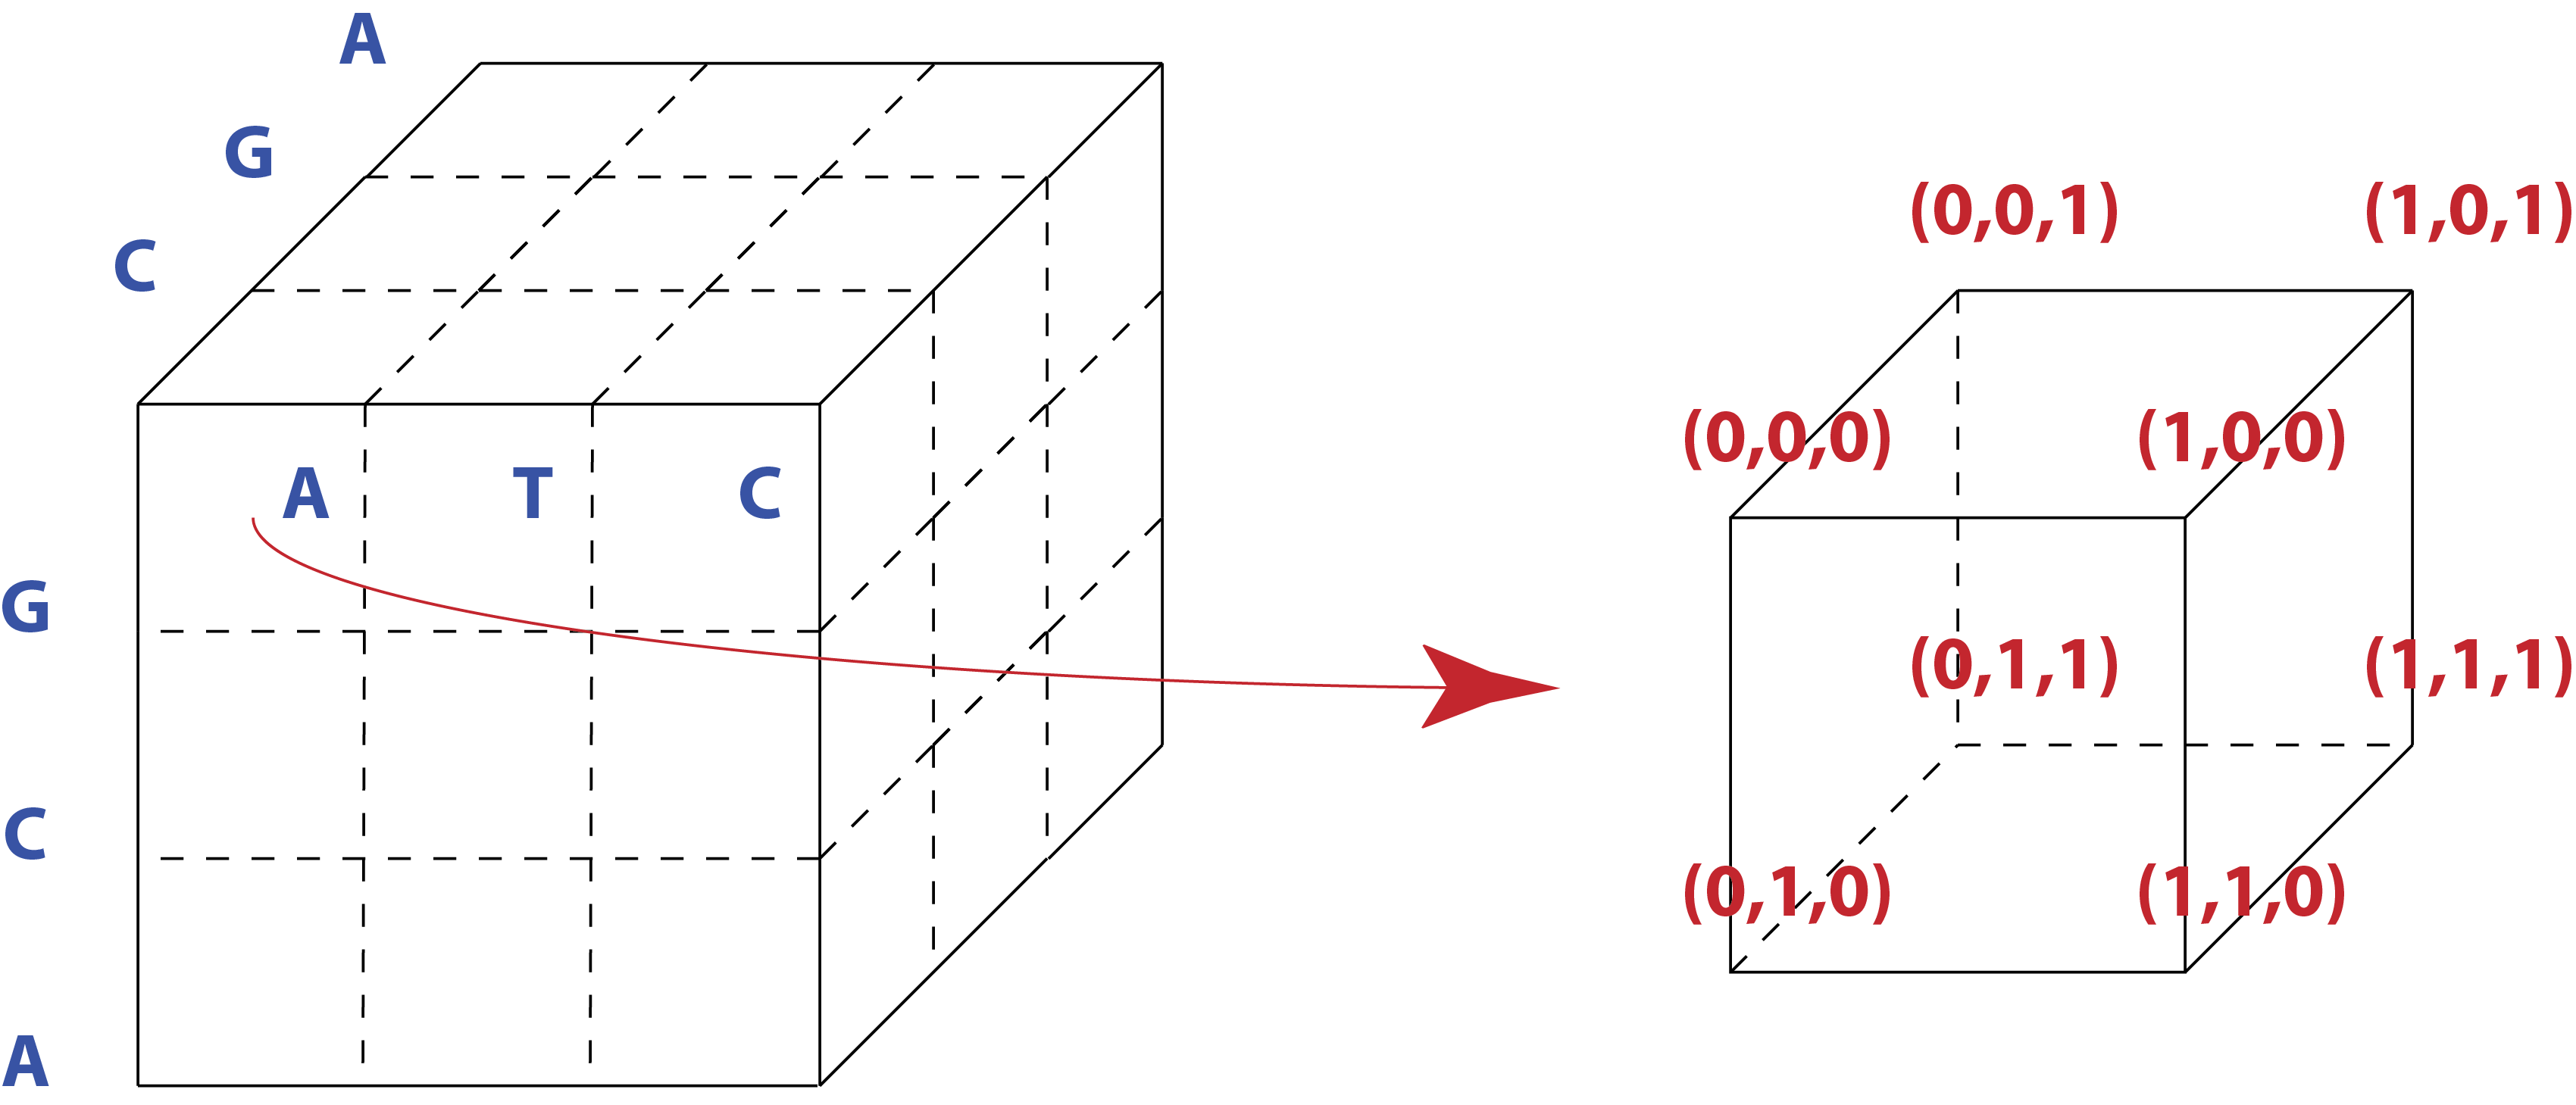
\includegraphics[width=0.5 \textwidth]{fig08/dp_mutiple_dimension.png}
  \caption{A three-dimensional DP array}
\end{figure}

%
% Example of alignment representation
%
\subsubsection*{Example of alignment representation}
\begin{figure}[H]
  \centering
      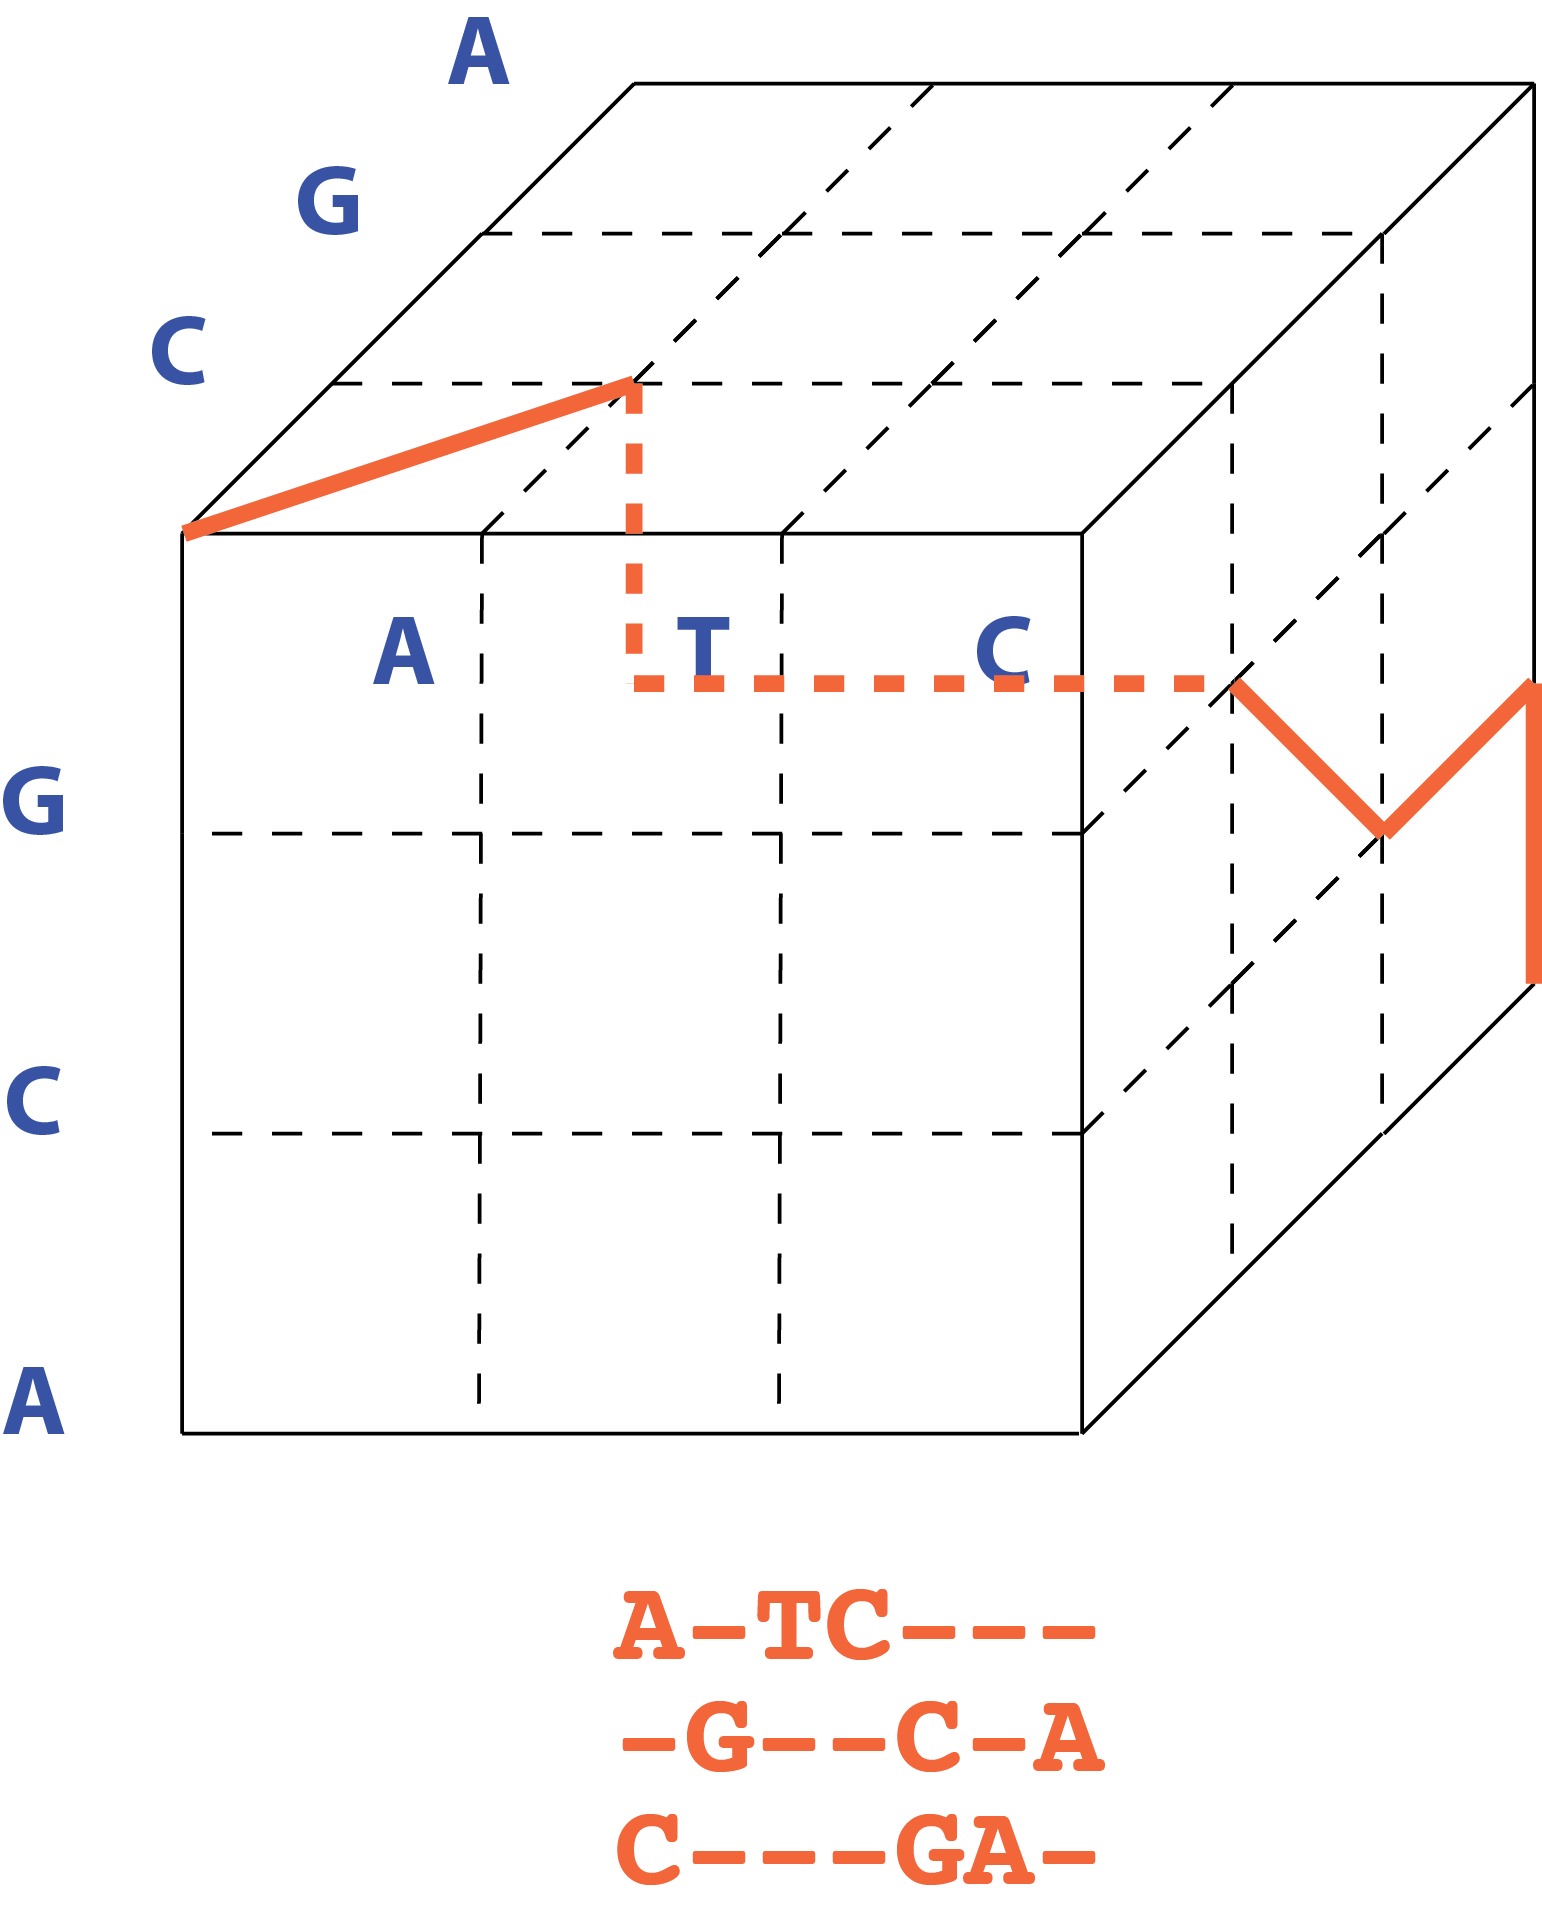
\includegraphics[width=0.2 \textwidth]{fig08/alignment_repsentation.png}
  \caption{An alignment with a three-dimensional DP array}
\end{figure}

%
% The number of candidate scores for a vertex 
%
\subsubsection*{The number of candidate scores for a vertex }
The number of the inbound neighboring vertices is defined as follows. 

\[
\sum_{i=0}^{m-1} \binom{m}{i}  = 2^m - 1
\]

%
% Example of edges of 3-dimensional cell
%
\subsubsection*{Example of edges of 3-dimensional cell}
\begin{figure}[H]
  \centering
      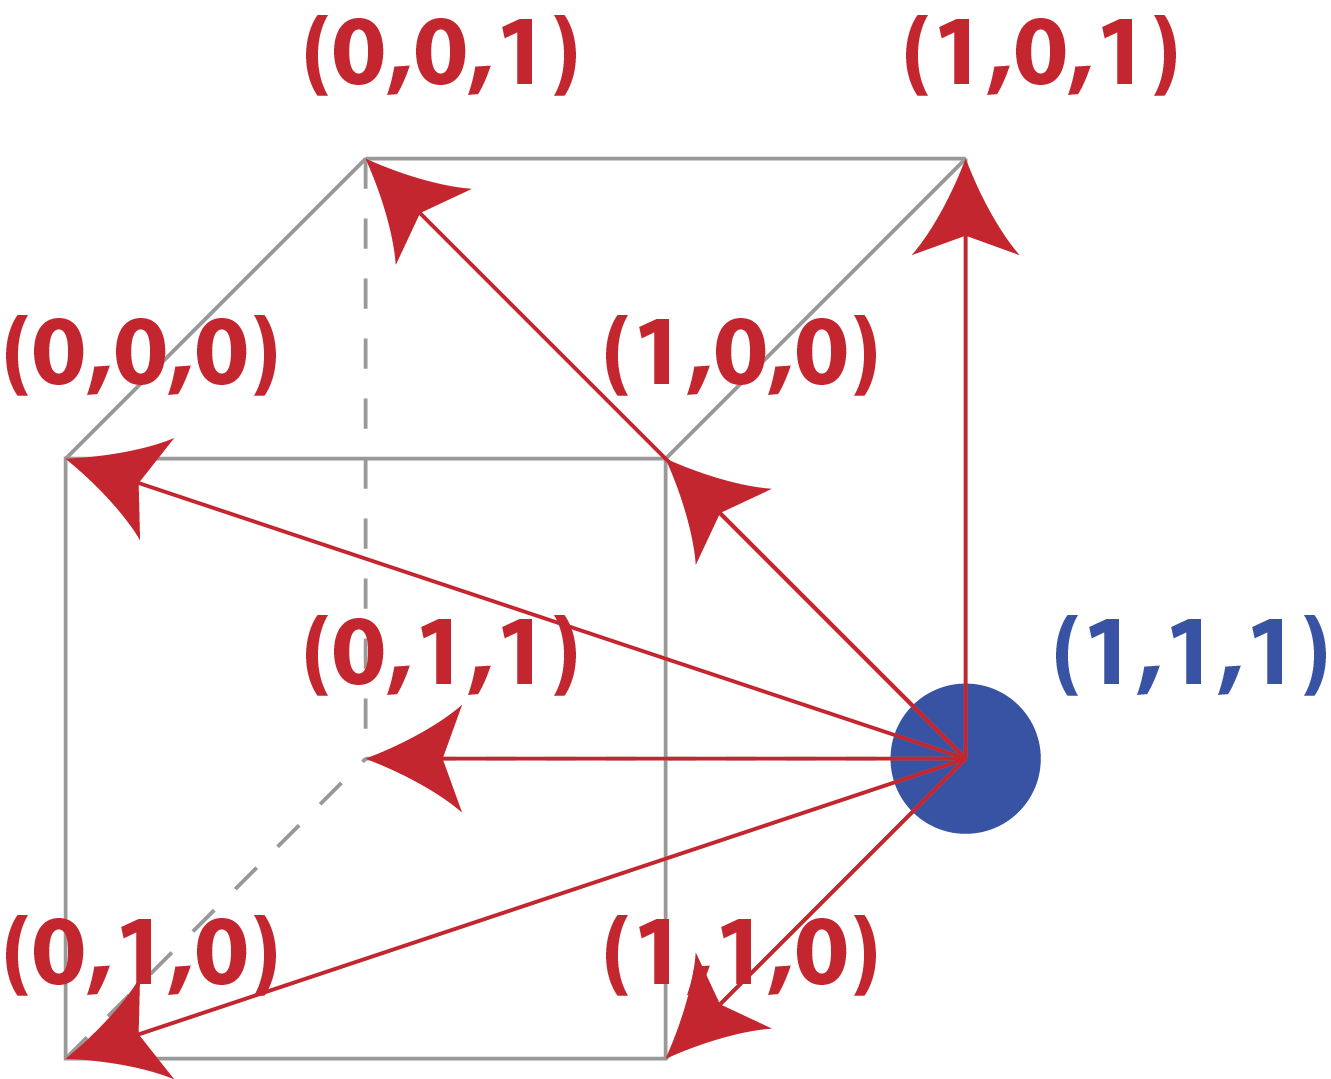
\includegraphics[width=0.25 \textwidth]{fig08/msa_vertex_index.png}
  \caption{An example of seven different edges to one vertex when m = 3}
\end{figure}

%
% A pruning method
%
\subsubsection*{A pruning method}
\begin{itemize}
\item $K$ : a score of an MSA (it does not need to be the optimal)
\item $\nu$ : current vertex
\item $S_{\nu}$ : best score from the start vertex to $\nu$ (by DP)
\item $F_{\nu}$ : best score from the end vertex to $\nu$ (by non-DP)
\item if $S_{\nu}$ + $F_{\nu} < K$ then $\nu$ does not lie on the optimal path
\end{itemize}

\begin{figure}[H]
  \centering
      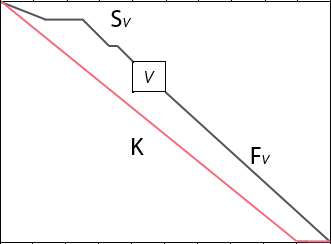
\includegraphics[width=0.3 \textwidth]{fig08/msa_table.png}
  \caption{Score estimation}
\end{figure}

%
% Forward-recursion DP for MSA
%
\subsubsection*{Forward-recursion DP for MSA}
Instead of looking up inbound neighboring vertices, the forward recursion DP sends the calculated score to all outbound neighboring vertices. 

\begin{figure}[H]
  \centering
      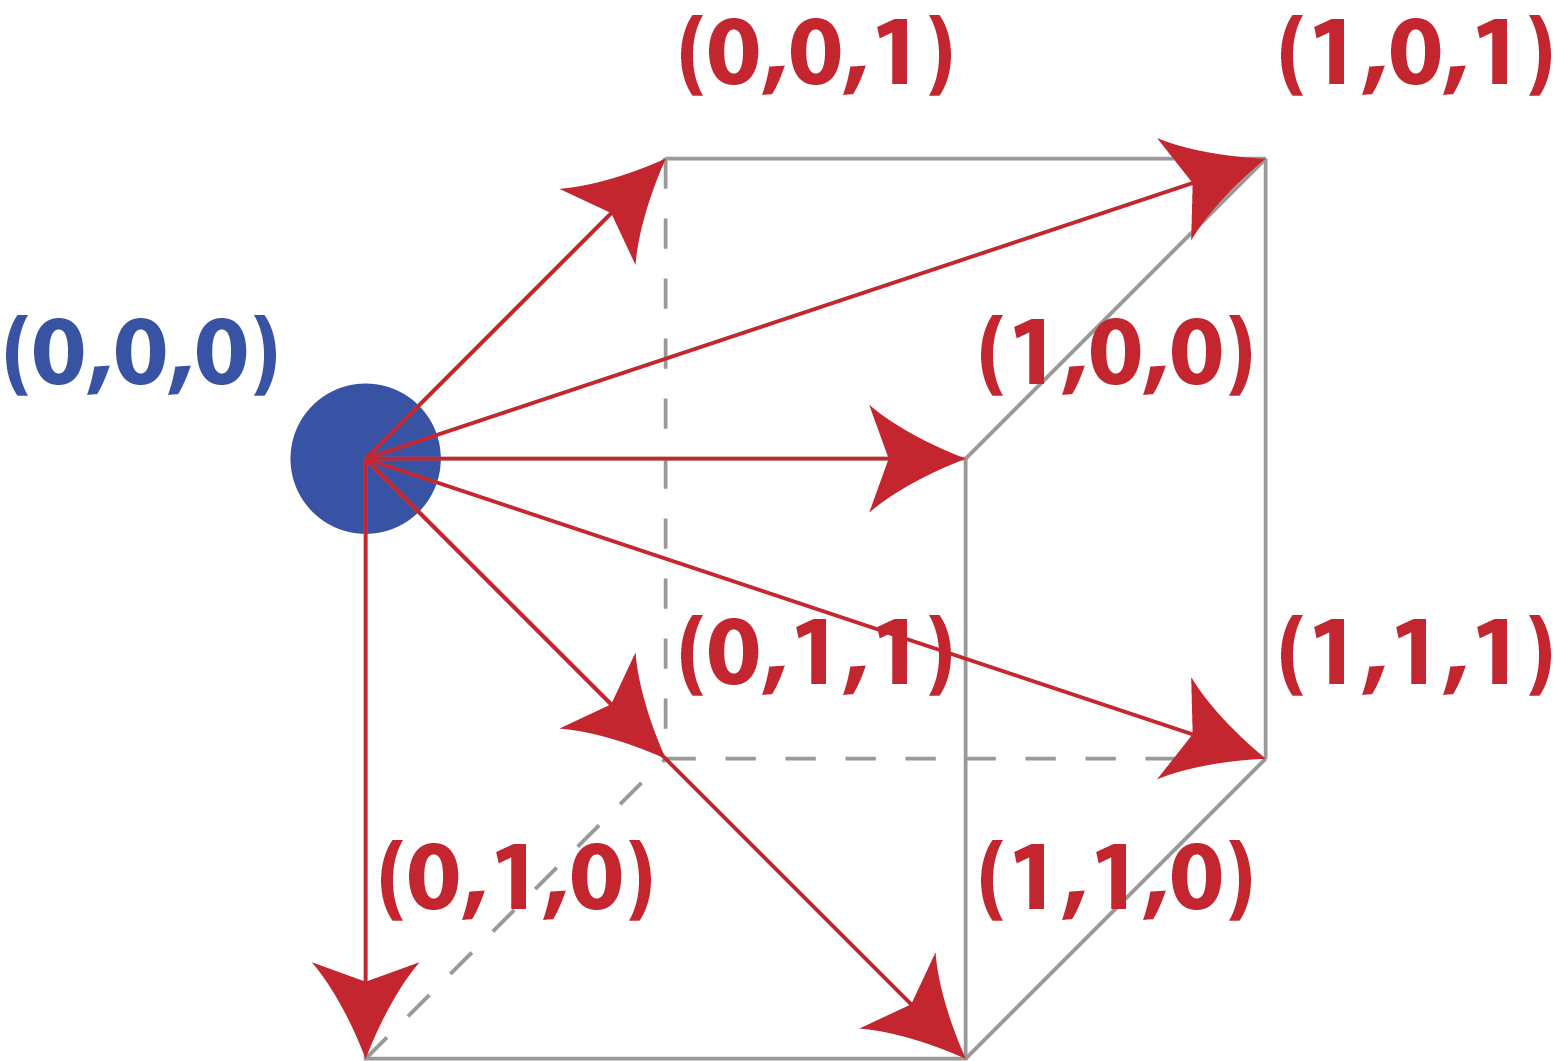
\includegraphics[width=0.3 \textwidth]{fig08/cell_update_msa_feedforward.png}
  \caption{Values are forwarded to all outgoing neighbors}
\end{figure}

\bigskip 

%\end{document}


\end{document}
